\documentclass{article}%
\usepackage[T1]{fontenc}%
\usepackage[utf8]{inputenc}%
\usepackage{lmodern}%
\usepackage{textcomp}%
\usepackage{lastpage}%
\usepackage[head=40pt,margin=0.5in,bottom=0.6in]{geometry}%
\usepackage{graphicx}%
%
\title{\textbf{ANC designó a Alfredo Ruíz como defensor del Pueblo}}%
\author{ERNESTO MENDEZ}%
\date{20/11/2018}%
%
\begin{document}%
\normalsize%
\maketitle%
\textbf{URL: }%
http://www.eluniversal.com/politica/26292/anc{-}designo{-}a{-}alfredo{-}ruiz{-}como{-}nuevo{-}defensor{-}del{-}pueblo\newline%
%
\textbf{Periodico: }%
EU, %
ID: %
26292, %
Seccion: %
politica\newline%
%
\textbf{Palabras Claves: }%
NO\_TIENE\newline%
%
\textbf{Derecho: }%
1.10, %
Otros Derechos: %
, %
Sub Derechos: %
1.10.2.1\newline%
%
\textbf{EP: }%
NO\newline%
\newline%
%
\textbf{\textit{El presidente órgano plenipotenciario, Diosdado Cabello, explicó que el nuevo titular de la entidad se encontraba ejerciendo funciones en ese mismo despacho, pero de manera temporal}}%
\newline%
\newline%
%
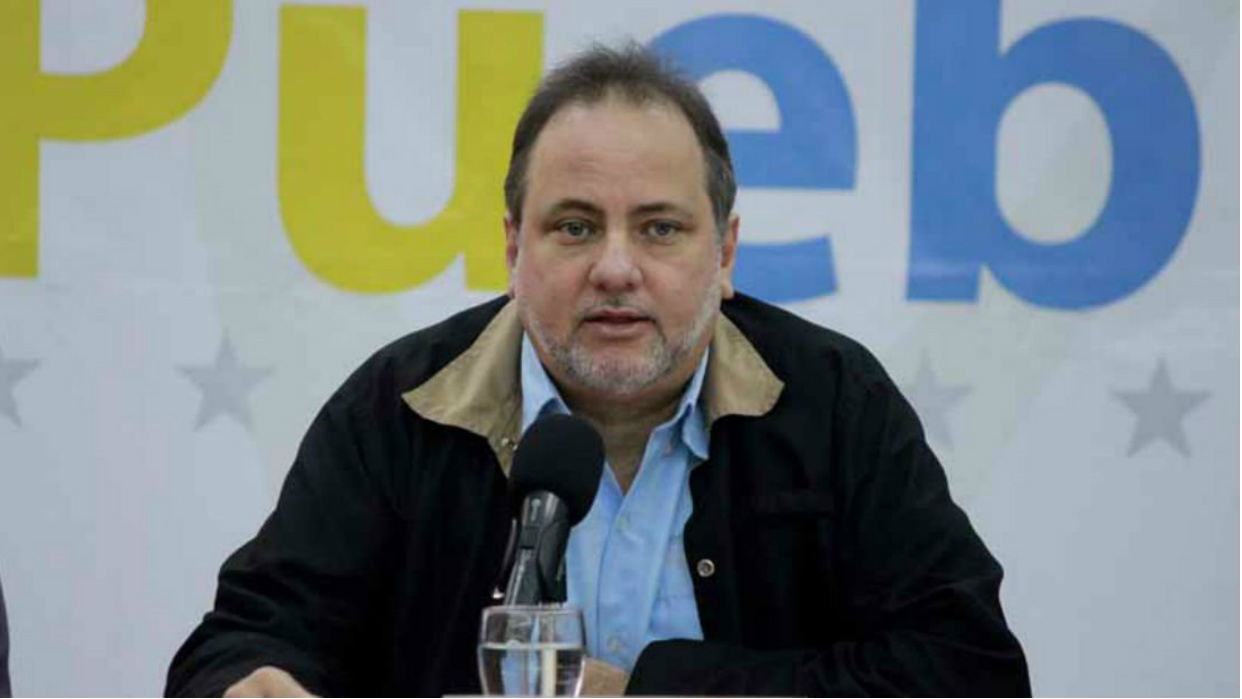
\includegraphics[width=300px]{5.jpg}%
\newline%
%
Caracas.{-} La Asamblea Nacional Constituyente (ANC) juramentó este martes a Alfredo Ruíz como nuevo defensor del Pueblo.%
\newline%
%
El presidente del órgano plenipotenciario, Diosdado Cabello, realizó una "moción de urgencia" en la sesión para designar a~Ruíz como titular de la Defensoría, puesto que se encontraba ejerciendo el cargo en ese mismo despacho de manera temporal.%
\newline%
%
\end{document}